5. Для нахождения области определения $f(x)$ необходимо решить неравенство\\ $\cfrac{x(x^2+x-12)(x^2-3x+2)}{(x^2-x-6)(-x+5)}\geqslant0
\Leftrightarrow \cfrac{x(x+4)(x-3)(x-2)(x-1)}{(x-3)(x+2)(-x+5)}\geqslant0.$ Решим его, применив метод интервалов:
$x\in[-4;-2)\cup[0;1]\cup[2;3)\cup(3;5).$
\begin{figure}[ht!]
\center{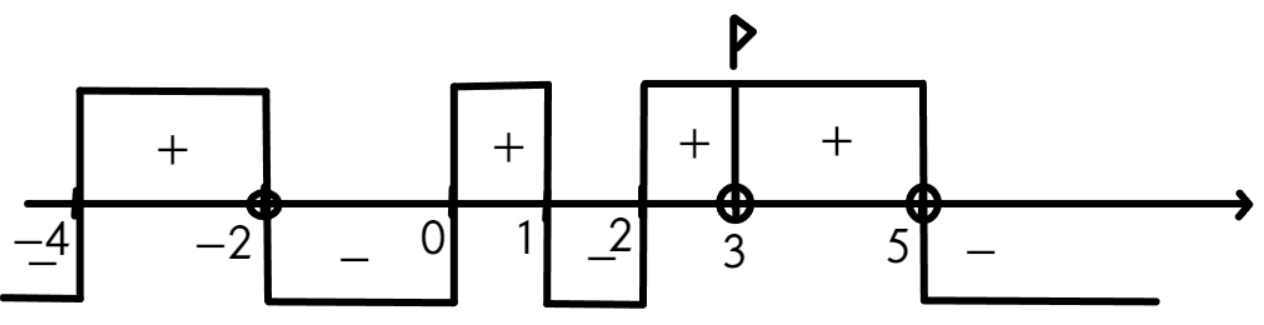
\includegraphics[scale=0.35]{isl9-5.png}}
\end{figure}\\
